\documentclass{beamer}

\mode<presentation>
{
  \usetheme{Frankfurt}
  \setbeamercovered{transparent}
  %\usecolortheme{whale}
}

\usepackage[english]{babel}
\usepackage[latin1]{inputenc}
\usepackage{times}
\usepackage[T1]{fontenc} 
% Or whatever. Note that the encoding and the font should match. If T1
% does not look nice, try deleting the line with the fontenc.
\usepackage{amsmath}
\usepackage{algorithmic}

\newcommand{\tab}[1]{\hspace{.2\textwidth}\rlap{#1}}

\newcommand{\linespace}{\vskip 0.25cm}

\definecolor{MyForestGreen}{rgb}{0,0.7,0} 
\newcommand{\tableemph}[1]{{#1}}
\newcommand{\tablewin}[1]{\tableemph{#1}}
\newcommand{\tablemid}[1]{\tableemph{#1}}
\newcommand{\tablelose}[1]{\tableemph{#1}}

\definecolor{MyLightGray}{rgb}{0.6,0.6,0.6}
\newcommand{\tabletie}[1]{\color{MyLightGray} {#1}}

% The text in square brackets is the short version of your title and will be used in the
% header/footer depending on your theme.
\title[Intrusion Detection]{Intrusion Detection with \\ Genetic Algorithms and Fuzzy Logic}

% Sub-titles are optional - uncomment and edit the next line if you want one.
% \subtitle{Why does sub-tree crossover work?} 

% The text in square brackets is the short version of your name(s) and will be used in the
% header/footer depending on your theme.
\author[Ireland]{Emma Ireland}

% The text in square brackets is the short version of your institution and will be used in the
% header/footer depending on your theme.
\institute[U of Minn, Morris]
{
  Division of Science and Mathematics \\
  University of Minnesota, Morris \\
  Morris, Minnesota, USA
}

% The text in square brackets is the short version of the date if you need that.
\date[December 7, 2013] % (optional)
{December 7, 2013 \\ UMM CSci Senior Seminar Conference}

% Delete this, if you do not want the table of contents to pop up at
% the beginning of each subsection:
\AtBeginSection[]
{
  \begin{frame}<beamer>
    \frametitle{Outline}
    \tableofcontents[currentsection, hideothersubsections]
  \end{frame}
}

\begin{document}

\begin{frame}
  \titlepage
\end{frame}

% For a 20-25 minute senior seminar talk you probably want something like:
% - Two or three major sections (other than the summary).
% - At *most* three subsections per section.
% - Talk about 30s to 2min per frame. So there should probably be between
%   15 and 30 frames, all told.

\section*{Overview}

\subsection*{The Big Picture}

\begin{frame}
  \frametitle{The Big Picture}
  \begin{itemize}
  	\item Computer lab gets large numbers of login attempts that are attempts at intrusion.
	\begin{itemize}
		\item Trying to gain root access to the system
		\item Delete files of users and change user passwords.
	\end{itemize}
	\linespace
	\linespace
	\linespace

	\item An attempt is an attack if there are more than \emph{n} number of attempts within \emph{t} time interval.
	\item Number of login attempts (for failed passwords or for users that don't exist) over period of 6 days (12/1 - 12/6):
	\begin{itemize}
		\item normal lab box (avenger): 1,834 attacks
		\item normal box, more recently added than avenger (kenshiro): 1,887 attacks
	\end{itemize}
  \end{itemize}
\end{frame}


\begin{frame}
  \frametitle{The Big Picture}
  \begin{itemize}
	\item With intrusion detection system (IDS): classify attempts.
	\item Intrusion detection systems provide a way of detecting attacks by monitoring network activities for malicious or abnormal behaviors then producing reports, alerts, actions.
	\item Training an IDS: use a fuzzy genetic algorithm.
  \end{itemize}
\end{frame}

\subsection*{Outline}

\begin{frame}
  \frametitle{Outline}
  \tableofcontents[hideallsubsections]
\end{frame}
%%%%%%%%%%%%%%%%%%%%%%%%%%%%%%%%%%%%%%%%%%%%%%%%%%%%%%%%%%%%%%%%%%%%%%%%%%%%%%%%%
%%%%%%%%%%%%%%%%%%%%%%%%%%%%%%%%%%%%%%%%%%%%%%%%%%%%%%%%%%%%%%%%%%%%%%%%%%%%%%%%%
%%%%%%%%%%%%%%%%%%%%%%%%%%%%%%%%%%%%%%%%%%%%%%%%%%%%%%%%%%%%%%%%%%%%%%%%%%%%%%%%%
%%%%%%%%%%%%%%%%%%%%%%%%%%%%%%%%%%%%%%%%%%%%%%%%%%%%%%%%%%%%%%%%%%%%%%%%%%%%%%%%%
\section[Intrusion Detection]{Intrusion Detection}
\subsection{Types of Networking Attacks}
\begin{frame}
  \frametitle{Types of Networking Attacks}
  \begin{itemize}
  	\item Denial of Service (DoS) - makes machine inaccessible to user by making it too busy to serve legitimate requests.
  	
  	\begin{itemize}
  		\item Systems lockout user from account after failed login attempts. 
  		\item Use this to prevent users from logging in, by failing to log in enough times to lock account.
  	\end{itemize}

  	\linespace
  	\linespace
  	\linespace
  	
  	\item Probe - examines machine to collect info about weaknesses, could be used to compromise system.
  	
  	\begin{itemize}
  		\item Trying to determine version of software is being run, if it has known issue it allows attacker to attempt to attack that.
  	\end{itemize}
  \end{itemize}
\end{frame}


\subsection{Detection Methodologies}
\begin{frame}
  \frametitle{Detection Methodologies}
  \begin{itemize}
  	\item Signature-based detection: compares well-known patterns of attacks
that are already known to IDS against captured events in order to identify possible attacks.
	\begin{itemize}
		\item Simple and effective way to detect known attacks, 
		
		ineffective against new kinds of unknown attacks.
	\end{itemize}

\linespace
\linespace
\linespace

  	\item Anomaly-based detection: looks for patterns of activity that are rare and uncommon.
	\begin{itemize}
		\item Harder to do than signature-based detection, 
		
		can be an effective way to detect new, unknown attacks.
	\end{itemize}
  \end{itemize}
\end{frame}


\subsection{Data Sets - KDD99 and RLD09}
\begin{frame}
  \frametitle{KDD99}
	\begin{itemize}
		\item Generated by simulating a military network environment in 1999.
		\item Has long been a standard data set for intrusion detection.
		
\linespace		
		
		\item Data was processed into 5 million \emph{records}.
			\begin{itemize}
				\item A record is a sequence of TCP packets, between which data flows to and from a source IP address to a target IP address.
			\end{itemize}
		\item Each record: classified as either normal or attack.
	\end{itemize}
\end{frame}


\begin{frame}
  \frametitle{Features of KDD99}
	\begin{itemize}
		\item KDD99 uses 41 \emph{features} - properties of record that are used to describe activity, help to distinguish normal connections from attacks.
		
		\linespace
		\linespace
		
		\item duration: length of the record in seconds.
		\item num\_failed\_logins: number of failed login attempts.
		\item root\_shell: returns 1 if root shell is obtained, else returns 0.
	\end{itemize}
\end{frame}



\begin{frame}
  \frametitle{RLD09}
	\begin{itemize}
		\item RLD09: created because KDD99 was 10 years old, 
		
		newer attack types not in KDD99 because of age.
		\item Data was captured from university in Bangkok, Thailand.
		\item Has normal network activity, and 17 different types of attacks
	\end{itemize}
\end{frame}



\begin{frame}
  \frametitle{Rules}
	\begin{itemize}
		\item A commonly used approach for detecting intrusions is to use rules.
		\item If-Then format: If (\emph{condition}) then (\emph{consequence}).
		\begin{itemize}
			\item Condition: one or more features
			\item Consequence: says if it is an intrusion or not.
			\linespace
			\item If \emph{duration $\leq$ 4} then \emph{intrusion}.
		\end{itemize}				
	\end{itemize}
\end{frame}



\begin{frame}
  \frametitle{Training and Testing Sets}
	\begin{itemize}
		\item Algorithm used runs risk of memorizing the data in training set, so important to keep some data separate, as unseen data for testing.
        \linespace
        \linespace
		\item Divide data set into 2 subsets: \emph{training set} and \emph{test set}.
        \item The given algorithm is trained on the training set to look for patterns.
        \item These patterns are then verified using the test set.
	\end{itemize}
\end{frame}



\subsection{Determining the Accuracy of an Algorithm}
\begin{frame}
  \frametitle{Determining the Accuracy of an Algorithm}
\begin{table}
Predicted
\begin{tabular}{l|ll}
Actual   & Not Attack & Attack \\ \hline
Not Attack & True Negative (TN) & False Positive (FP) \\
Attack & False Negative (FN) & True Positive (TP)  \\
\end{tabular}
\end{table}
\linespace
\linespace
\begin{center}
Detection rate (DR): percentage of normal and attack activity correctly classified from the total number of data records.
\end{center}
\end{frame}
%%%%%%%%%%%%%%%%%%%%%%%%%%%%%%%%%%%%%%%%%%%%%%%%%%%%%%%%%%%%%%%%%%%%%%%%%%%%%%%%%
%%%%%%%%%%%%%%%%%%%%%%%%%%%%%%%%%%%%%%%%%%%%%%%%%%%%%%%%%%%%%%%%%%%%%%%%%%%%%%%%%
\section[Fuzzy Classification]{Fuzzy Classification}
\subsection{Fuzzy Logic}
\begin{frame}
	\frametitle{Fuzzy Logic}
	\begin{itemize}
		\item Fuzzy logic: used in intrusion detection systems to find degree of certainty of record being attack.
			\begin{itemize}
				\item If it's not clear if activity is an attack, fuzzy logic says where on a spectrum it is and how certain it is of being an attack.
			\end{itemize}
		\linespace
		\linespace
		\linespace
		\item Fuzzy logic rules: similar to rules described before, except that
consequence is certainty factor. 
		\begin{itemize}
			\item If (\emph{duration} = 6.2) then (\emph{the degree of certainty of the record being an attack is 0.8}).
		\end{itemize}
	\end{itemize}
\end{frame}

\subsection{Finding the Degree of Certainty}
\begin{frame}
  \frametitle{Trapezoidal Shape}
	\begin{itemize}
		\item Used to decide how certain a record is of being an attack.
		\item Described with 4 numbers that are used to determine what the trapezoid looks like.
		\begin{center}
		  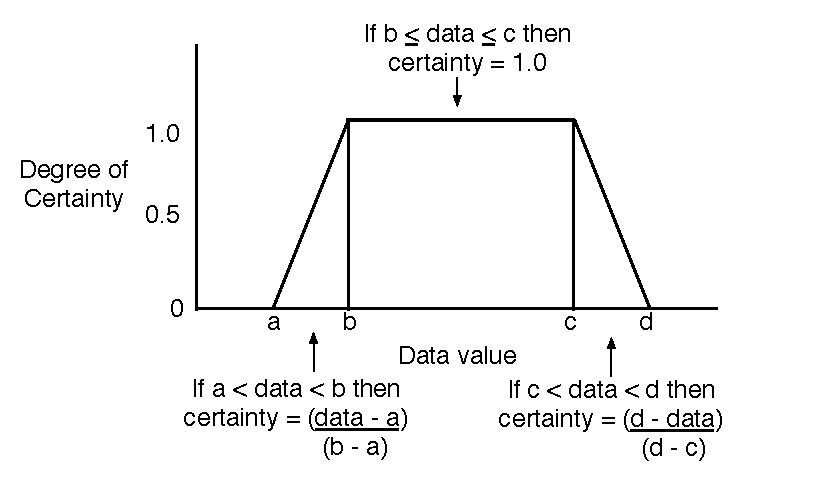
\includegraphics[width=0.85\textwidth]{../trapFigTemplate.pdf}		
		\end{center}
		\item Certain in middle, not as certain in triangle areas.
	\end{itemize}
\end{frame}



\begin{frame}
  \frametitle{Finding the Degree of Certainty of a Record Being an Attack}
	Suppose that the feature is duration, and it is 6.2 seconds. Then data=6.2.
  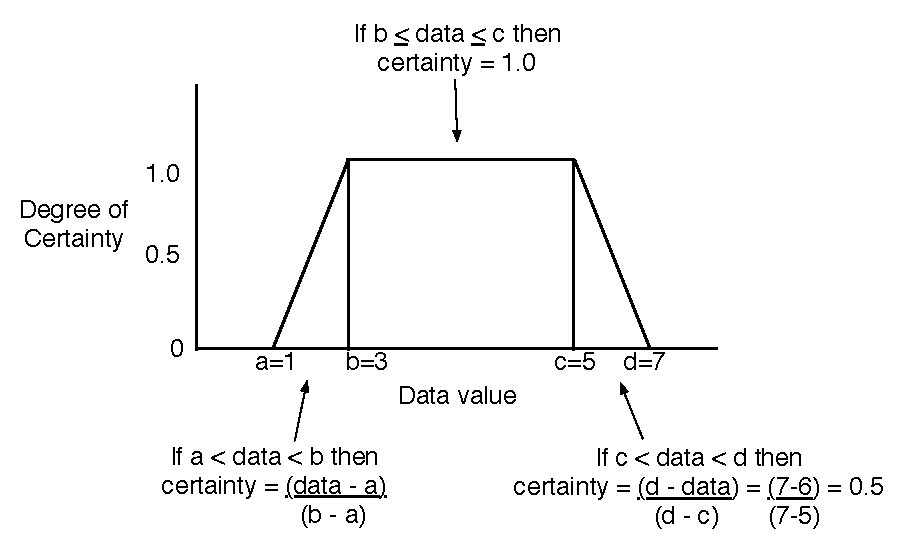
\includegraphics[width=0.95\textwidth]{../trapFigExample.pdf}
\end{frame}


\subsection{Encoding of Features and Rules}
\begin{frame}
	\frametitle{Encoding of Features and Rules}
	\begin{itemize}
	\item Four parameters are encoded into blocks. Each block is feature with values 0-7.
	\item Rule has 1 block for each of 12 features followed at end by marker indicating type of attack.
	\end{itemize}

\begin{figure}
\begin{small}
\begin{tabular}{|cccc|c|cccc|c|} \hline
010 & 011 & 100 & 101   & ... & 001 & 100 & 101 & 111   & Attack\\
a=2 & b=3 & c=4 & d=5   & ... & a=1 & b=4 & c=5 & d=7   &\\  
    &     & Block 1&    &        &     & Block 12& &       & Type\\
\hline\end{tabular}
\caption{Based on [Jongsuebsuk \emph{et al.}, 2013]}
\end{small}
\end{figure}
\end{frame}


\begin{frame}
	\frametitle{Encoding of Features and Rules}
\begin{figure}
\begin{small}
\begin{tabular}{|cccc|c|cccc|c|} \hline
010 & 011 & 100 & 101   & ... & 001 & 100 & 101 & 111   & Attack\\
a=2 & b=3 & c=4 & d=5   & ... & a=1 & b=4 & c=5 & d=7   &\\ 
    &     & Block 1&    &        &     & Block 12& &       & Type\\
\hline\end{tabular}
\end{small}
\end{figure}
\tab{$\downarrow$} \tab{} \tab{} \tab{$\downarrow$}
  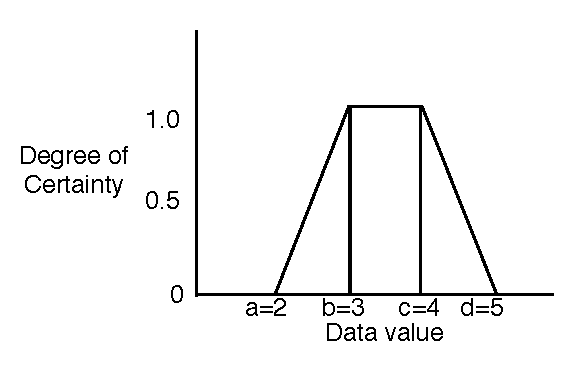
\includegraphics[width=0.50\textwidth]{../Talk/MutCrossTrapezoids/mut2345.pdf}
  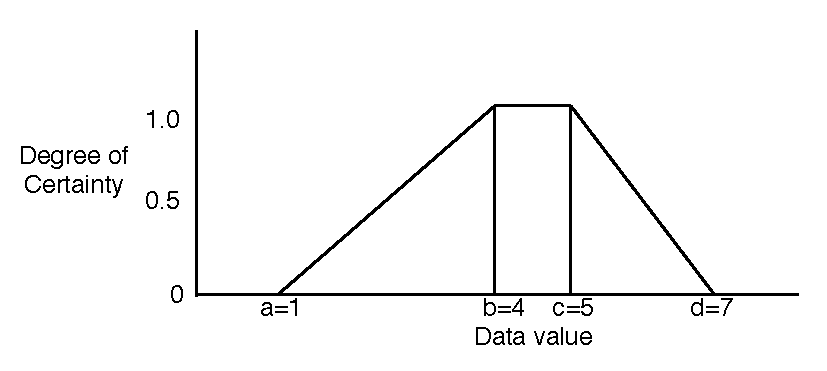
\includegraphics[width=0.58\textwidth]{../Talk/MutCrossTrapezoids/cross1457.pdf}

Degree of certainty is computed for each of 12 blocks, if sum of those is greater than a threshold, declared as attack.
\end{frame}
%%%%%%%%%%%%%%%%%%%%%%%%%%%%%%%%%%%%%%%%%%%%%%%%%%%%%%%%%%%%%%%%%%%%%%%%%%%%%%%%%
%%%%%%%%%%%%%%%%%%%%%%%%%%%%%%%%%%%%%%%%%%%%%%%%%%%%%%%%%%%%%%%%%%%%%%%%%%%%%%%%%
\section[Genetic Algorithms]{Genetic Algorithms}
\subsection{GA Overview}
\begin{frame}
  \frametitle{Genetic Algorithms}
	\begin{itemize}
		\item GAs: search technique used to find solutions to problems.
        \item Possible solutions to problems: represented in a variety of problem dependent ways.
        
        \begin{itemize}
        	\item IDS rules are represented as bit strings.
        \end{itemize}
        
        \linespace
        \item A randomly generated population of potential solutions is created. Mutation, crossover, selection applied to each generation until acceptable solution is found or time limit is exceeded.
	\end{itemize}
\end{frame}


\subsection{Mutation and Crossover}
\begin{frame}
  \frametitle{Mutation}
Mutation: random bits in an individual, or possible solution, are randomly changed. Mutation takes bits of rule and changes them to form slightly different rule.

\begin{figure}
\begin{small}
	\begin{tabular}{|cccc|} \hline
	010 & 011 & 100 & \textbf{101}\\
	a=2 & b=3 & c=4 & \textbf{d=5}\\
	\hline\end{tabular}
	$\rightarrow$
	\quad
	\begin{tabular}{|cccc|} \hline
	010 & 011 & 100 & \textbf{111}\\
	a=2 & b=3 & c=4 & \textbf{d=7}\\
	\hline\end{tabular}
\end{small}
\end{figure}

	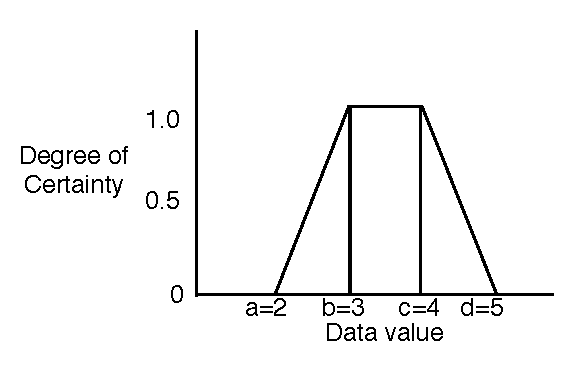
\includegraphics[width=0.50\textwidth]{../Talk/MutCrossTrapezoids/mut2345.pdf}
	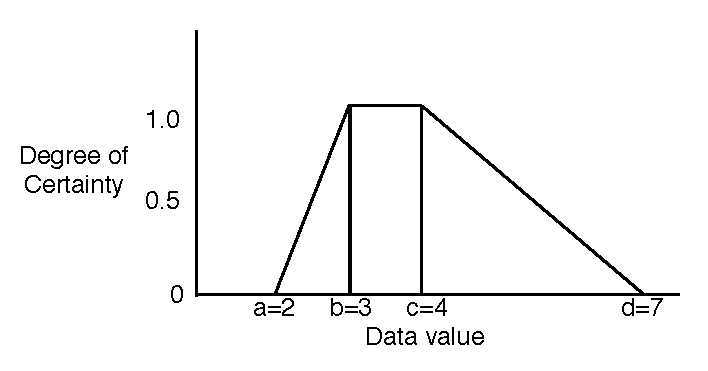
\includegraphics[width=0.55\textwidth]{../Talk/MutCrossTrapezoids/mut2347.pdf}
	
After mutation: transition from c to d is more gradual.
\end{frame}


\begin{frame}
  \frametitle{Crossover}
  \begin{itemize}
  	\item Crossover: two individuals swap sequences of bits to form two new individuals.
  	\item In IDS: crossover takes 2 rules and creates new rules by swapping bits of old rules.
  \end{itemize}
\end{frame}


\begin{frame}
  \frametitle{Crossover}
\begin{figure}
\begin{small}
\textbf{Before}
	\begin{tabular}{|cccc|} \hline
	001 & \textbf{011} & 101 & 111\\
	a=1 & \textbf{b=3} & c=5 & d=7\\
	\hline\end{tabular}
	\quad
	\begin{tabular}{|cccc|} \hline
	010 & \textbf{100} & 110 & 111\\
	a=2 & \textbf{b=4} & c=6 & d=7\\
	\hline\end{tabular}
\end{small}
\end{figure}
	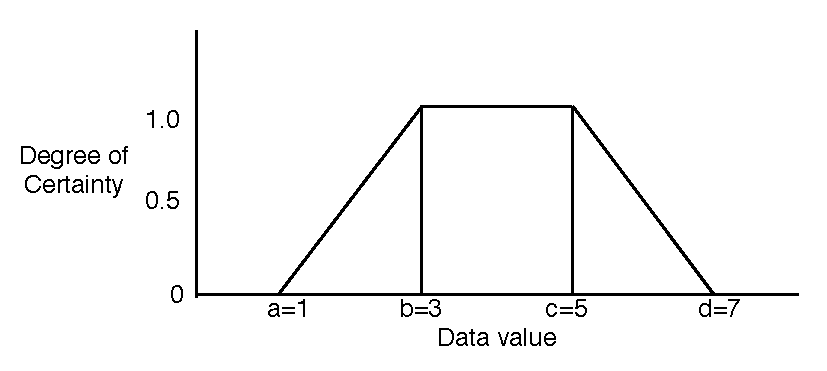
\includegraphics[width=0.50\textwidth]{../Talk/MutCrossTrapezoids/cross1357.pdf}
	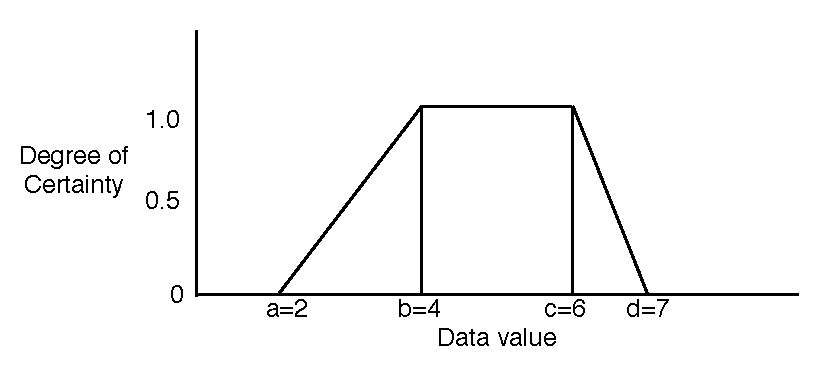
\includegraphics[width=0.55\textwidth]{../Talk/MutCrossTrapezoids/cross2467.pdf}
	
\begin{figure}
\begin{small}
\textbf{After}
	\begin{tabular}{|cccc|} \hline
	001 & \textbf{100} & 101 & 111\\
	a=1 & \textbf{b=4} & c=5 & d=7\\
	\hline\end{tabular}
	\quad
	\begin{tabular}{|cccc|} \hline
	010 & \textbf{011} & 110 & 111\\
	a=2 & \textbf{b=3} & c=6 & d=7\\
	\hline\end{tabular}
\end{small}
\end{figure}
	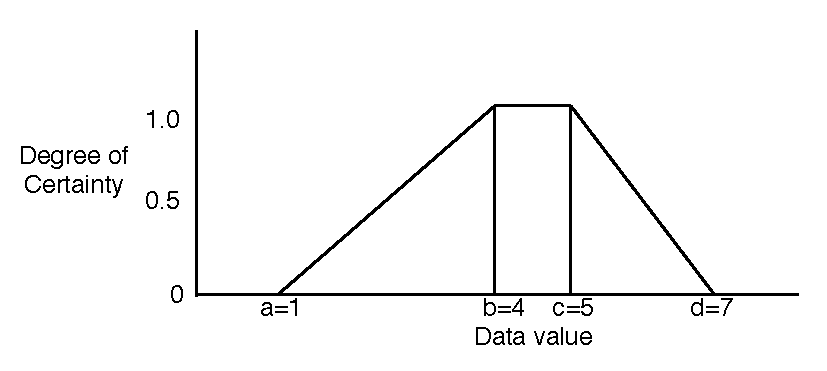
\includegraphics[width=0.50\textwidth]{../Talk/MutCrossTrapezoids/cross1457.pdf}
	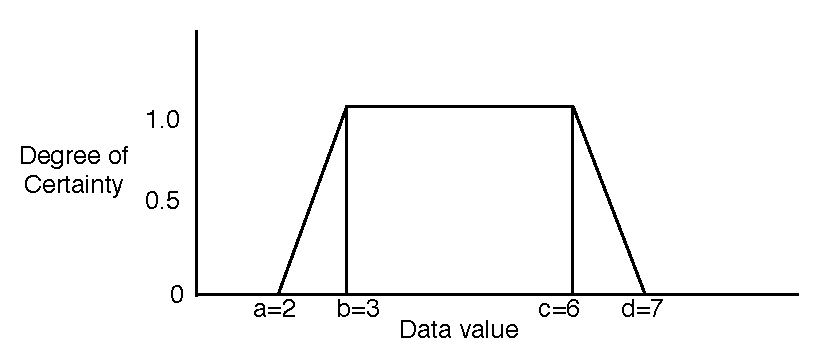
\includegraphics[width=0.55\textwidth]{../Talk/MutCrossTrapezoids/cross2367.pdf}
\end{frame}


\subsection{Selection and Fitness}
\begin{frame}
  \frametitle{Selection and Fitness}
	\begin{itemize}
        \item Selection: individuals that have better fitness are chosen to be parents.
        \item Fitness of individual is specified by fitness function, which determines quality of particular individual.
        
        \linespace
        \linespace
        
       	\item In an IDS: fitness measures how well a rule classifies records as either attacks or normal activity. Selection combined with fitness function directs search towards effective solution.
	\end{itemize}
\end{frame}


\begin{frame}
	\frametitle{Fitness function}
	The fitness function to be maximized is:
	\begin{equation*}
	\frac{\alpha}{A} - \frac{\beta}{B}
	\end{equation*}

	$\alpha$: \# of attack records correctly identified as attack.

	$A$: \# of attack records.

	$\beta$: \# of normal records incorrectly classified as attack.
	
	$B$: \# of normal records.

\linespace
\linespace
\linespace
\linespace
Best possible value of $\beta$ is 0.
It's good if $\alpha$ = $A$.

Best possible fitness value is 1.
\end{frame}
%%%%%%%%%%%%%%%%%%%%%%%%%%%%%%%%%%%%%%%%%%%%%%%%%%%%%%%%%%%%%%%%%%%%%%%%%%%%%%%%%
%%%%%%%%%%%%%%%%%%%%%%%%%%%%%%%%%%%%%%%%%%%%%%%%%%%%%%%%%%%%%%%%%%%%%%%%%%%%%%%%%
%%%%%%%%%%%%%%%%%%%%%%%%%%%%%%%%%%%%%%%%%%%%%%%%%%%%%%%%%%%%%%%%%%%%%%%%%%%%%%%%%
%%%%%%%%%%%%%%%%%%%%%%%%%%%%%%%%%%%%%%%%%%%%%%%%%%%%%%%%%%%%%%%%%%%%%%%%%%%%%%%%%
\section[Experiments and Results]{Experiments and Results}
\subsection{Two Experiments using Only RLD09}
\begin{frame}
	\frametitle{Experiments Using Only RLD09}
	Experiment 1
	\begin{itemize}
		\item Fuzzy GA was used to create DoS and probe detection rules. 
		
		\item Both rules were then used together in testing process to identify attacks from testing data set.
		
		\linespace
		\linespace
		
		\item If record is classified as either DoS rule or Probe rule, it is classified as attack; else normal.

		\linespace
		\linespace
		
		\item Training set: 10,000 records.
		
		Test set: 26,500 records.
\end{itemize}
\end{frame}


\begin{frame}
	\frametitle{Experiments Using Only RLD09}
	Experiment 1 Results
\begin{table}
\begin{small}
\begin{tabular}{lllllll}
 & Attack & Normal & Total & FP(\%) & FN(\%) & DR(\%)\\
DoS Training & 1499 & 8501 & 10000 & 1.46 & 47.50 & 91.64\\
Probe Training & 2496 & 7504 & 10000 & 1.83 & 15.38 & 94.79\\
Testing & 10500 & 16000 & 26500 & 1.13 & 4.10 & 97.92\\
\end{tabular}
\end{small}
\end{table}

\linespace
Testing has:
\begin{itemize}
	\item Higher DR: IDS is more likely to classify attacks because it can match either attack type.
	\item Lower FN: IDS is less likely to predict that it's not an attack when it really is.
\end{itemize}
\end{frame}


\begin{frame}
	\frametitle{Experiments Using Only RLD09}
Experiment 2
	\begin{itemize}
		\item Attacks pulled out of training set, kept for unknown data testing, to test that fuzzy GA could detect unknown attacks.
		\item Fuzzy GA and decision tree algorithm, which is another common algorithm for classification problems.
		\item 7 tests were run. Each test case: 13 attack types plus normal activity that were in training set. 
		
		3 attack types used for unknown testing data set.
		\item Anomaly-based detection
	\end{itemize}
\end{frame}


\begin{frame}
	\frametitle{Experiments Using Only RLD09}
	Experiment 2 Results (7 tests were run in total, 5 are shown here.)
	
\begin{table}
\begin{footnotesize}
\begin{tabular}{llll}
Test & Unknown & Decision & Fuzzy\\
Case & Attacks & Tree DR (\%) & Genetic DR (\%)\\ \hline

1 & Adv Port Scan (Probe) & Avg = & Avg =\\
  & Ack Scan (Probe)                 & 98.33 & 100\\
  & Xmas Tree (Probe)                 &                 &\\ \hline

2 & UDP Flood (DoS) & Avg = & Avg =\\
  & Host Scan (Probe) & 46.65 & 99.80\\
  & UDP Scan (Probe) & &\\ \hline

3 & Jping (DoS) & Avg = & Avg =\\
  & Syn Scan (Probe) & 99.70 & 98.75\\
  & Fin Scan (Probe) & &\\ \hline

4 & UDP Flood (DoS) & Avg = & Avg =\\
  & RCP Scan (Probe) & 70.35 & 98.15\\
  & Fin Scan (Probe) & &\\ \hline

5 & Http Flood (DoS) & Avg = & Avg =\\
  & RCP Scan (Probe) & 99.94 & 97.50\\
  & Fin Scan (Probe) & &\\
\hline\end{tabular}
\end{footnotesize}
\end{table}
\end{frame}



\subsection{Three Experiments using Both RLD09 and KDD99}
\begin{frame}
	\frametitle{Experiments Using Both RLD09 and KDD99}
Three experiments used both RLD09 and KDD99.

\linespace
\linespace

Experiment 1 - Used fuzzy GA to classify normal activity and attacks from KDD99 and RLD09.
	
\begin{table}
\begin{tabular}{cccccc}
Data set & Attack & Normal & FP (\%) & FN (\%) & DR (\%)\\ \hline
KDD99 & 160,117 & 39,337 & 0.13 & 1.55 & 98.72\\
RLD09 & 10,500 & 16,000 & 1.14 & 3.39 & 97.97\\
\end{tabular}
\end{table}
\end{frame}


\begin{frame}
	\frametitle{Experiments Using Both RLD09 and KDD99}
Experiment 2
	\begin{itemize}
		\item Used the fuzzy GA to classify types of attacks in KDD99.
		\item 10 tests were run in total, 5 are shown here.
	\end{itemize}
\begin{table}
\begin{tabular}{cccccc}
Test & Attack & Type & FP (\%) & FN (\%) & DR (\%)\\ \hline
1 & Back & DoS & 85.33 & 0.00 & 16.56\\
2 & PoD & DoS & 84.66 & 0.00 & 15.58\\
3 & Smurf & DoS & 0.76 & 0.10 & 99.73\\
4 & Portsweep & Probe & 6.40 & 0.00 & 93.66\\
5 & Satan & Probe & 0.74 & 3.75 & 99.22\\
\end{tabular}
\end{table}

\begin{itemize}
	\item 8 test cases had DR greater than 93\%. Only 2 cases had low DR, (cases 1 and 2).
\end{itemize}

\end{frame}


\begin{frame}
	\frametitle{Experiments Using Both RLD09 and KDD99}
Experiment 3
	\begin{itemize}
		\item Used the fuzzy GA to classify types of attacks in RLD09.
		\item 17 tests were run in total, 6 are shown here.
	\end{itemize}
\begin{table}
\begin{tabular}{cccccc}
Test & Attack & Type & FP (\%) & FN (\%) & DR (\%)\\ \hline
1 & HTTP Flood & DoS & 0.36 & 3.5 & 99.46\\
2 & Smurf & DoS & 0.02 & 0 & 99.98\\
3 & UDP Flood & DoS & 11.06 & 0 & 89.59\\
4 & Fin Scan & Probe & 2.58 & 0 & 97.50\\
5 & IP Scan & Probe & 13.01 & 16.4 & 86.89\\
6 & Syn Scan & Probe & 0.65 & 4.2 & 99.24\\
\end{tabular}
\end{table}

\begin{itemize}
	\item 15 cases had DR greater than 97\%. 2 cases had lower DR, (cases 3 and 5).
\end{itemize}

\end{frame}
%%%%%%%%%%%%%%%%%%%%%%%%%%%%%%%%%%%%%%%%%%%%%%%%%%%%%%%%%%%%%%%%%%%%%%%%%%%%%%%%%
%%%%%%%%%%%%%%%%%%%%%%%%%%%%%%%%%%%%%%%%%%%%%%%%%%%%%%%%%%%%%%%%%%%%%%%%%%%%%%%%%
%%%%%%%%%%%%%%%%%%%%%%%%%%%%%%%%%%%%%%%%%%%%%%%%%%%%%%%%%%%%%%%%%%%%%%%%%%%%%%%%%
%%%%%%%%%%%%%%%%%%%%%%%%%%%%%%%%%%%%%%%%%%%%%%%%%%%%%%%%%%%%%%%%%%%%%%%%%%%%%%%%%
\section[Conclusions]{Conclusions}

\begin{frame}
\frametitle{Conclusions}
	\begin{itemize}
		\item The fuzzy genetic algorithm had a higher detection rate than a decision tree algorithm in most cases.
		\item Fuzzy genetic algorithms are good at detecting unknown attacks.
		\begin{itemize}
			\item Fuzzy GA DR: 99.8\%, Decision Tree DR: 46.7\%
		\end{itemize}

		\item The use of fuzzy genetic algorithms in intrusion detection is an effective way of detecting attacks - DR in all experiments was in the high 90s.
	\end{itemize}
\end{frame}


\begin{frame}
	\frametitle{Thanks!}
	
	Thank you for your time and attention!
		
	\linespace
	\linespace
	
	\begin{center}
	{\Large Questions?}
	\end{center}
\end{frame}


\section*{References}

\begin{frame} 
	\frametitle{References} 
	
	\begin{thebibliography}{lskdjf}
	
	\begin{small}
	\bibitem{6496342}
Jongsuebsuk, P. and Wattanapongsakorn, N. and Charnsripinyo, C.
\newblock Network intrusion detection with Fuzzy Genetic Algorithm for unknown attacks.
\newblock In \emph{2013 International Conference on Information Networking (ICOIN)}, pages 1-5, 2013.
	
	
	\bibitem{6559603}
Jongsuebsuk, P. and Wattanapongsakorn, N. and Charnsripinyo, C.
\newblock Real-time intrusion detection with fuzzy genetic algorithm.
\newblock In \emph{2013 10th International Conference on Electrical Engineering/Electronics, Computer, Telecommunications and Information Technology (ECTI-CON)}, pages 1-6, 2013.
	\end{small}
	
  	\end{thebibliography}
  	
  	\linespace
  	
  	\begin{center}
  	\begin{small}
  	See my Senior Seminar paper for additional references.
  	\end{small}
  	\end{center}
	
\end{frame} 


\begin{frame}
	\frametitle{DoS Attacks}
	\begin{itemize}
		\item Back: Attacker submits requests with URL's containing many front slashes. As server tries to process these requests it will slow down, becomes unable to process other requests.
		\linespace
		\linespace
		\item PoD: involves sending a malformed/malicious ping to computer. Historically, many systems could not handle a ping packet larger than the maximum IPv4 packet size (65,535 bytes). Sending a ping of this size could crash the target computer.
	\end{itemize}
\end{frame}


\begin{frame}
	\frametitle{Features of KDD99}
	\begin{itemize}
	\begin{small}
  \item src\_bytes: number of bytes sent from source to destination. Source is user who may or may not be attacker, destination is server being potentially attacked.

  \linespace
  \linespace
  
  \item serror\_rate: percentage of connections that have ``SYN" errors. When client attempts to connect to server, it first sends a SYN (synchronize) message to server. The server then acknowledges the request by sending a SYN-ACK to client. The connection is established when client sends an ACK back to server. A SYN error is a failure to get an ACK back.
  \end{small}
	\end{itemize}
\end{frame}


\end{document}


